\documentclass{article}
\usepackage{tikz, comment}
\usepackage{pifont}
\usepackage{fontspec}
\usetikzlibrary{arrows, decorations.markings, decorations.pathreplacing}
\begin{comment}
:Title: Not defined yet
:Tags: pi;;sine, sin ;area using polar coordinates, polar integral formula ;moment;polar form of a complex number
:Prob: 0.4135;0.3766;0.3631;0.3572;0.348
:Slug: No name yet

Description Here.........
\end{comment}
\begin{document}\centering

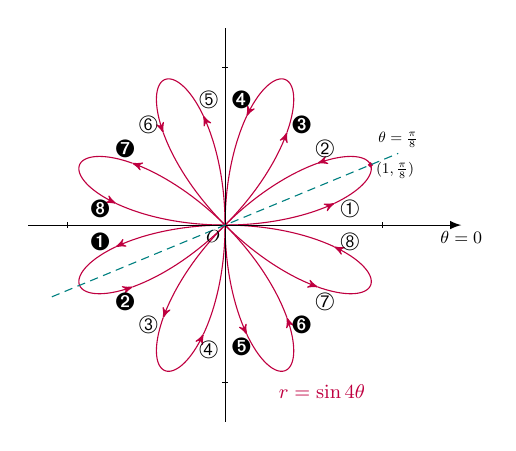
\begin{tikzpicture}[>=latex,xscale=.5*2*2, yscale=.5*2*2][font=\sf\small]

%\draw[xstep=1cm,ystep=1cm,color=gray!80] (0, -1) grid (8, 8);

\draw[->, >=stealth', purple, samples=100, smooth, domain=0:pi/16, variable=\t]
plot ({sin(4*\t r)*cos(\t r)}, {sin(4*\t r)*sin(\t r)}) -- ({sin(4*(pi/16) r)*cos(pi/16 r)}, {sin(4*(pi/16) r)*sin(pi/16 r)});

\foreach \n in {1,3,...,29}
\draw[->, >=stealth', purple, samples=100, smooth, domain=(\n)*pi/16:(\n+2)*pi/16, variable=\t]
plot ({sin(4*\t r)*cos(\t r)}, {sin(4*\t r)*sin(\t r)}) -- ({sin(4*((\n+2)*pi/16) r)*cos((\n+2)*pi/16 r)}, {sin(4*((\n+2)*pi/16) r)*sin((\n+2)*pi/16 r)});

\draw[purple, samples=150, smooth, domain=31*pi/16:2*pi, variable=\t]
plot ({sin(4*\t r)*cos(\t r)}, {sin(4*\t r)*sin(\t r)});

\draw[purple, fill, xscale=1/4, yscale=1/4] ({sin(4*(pi/8) r)*cos((pi/8) r)*4}, {sin(4*(pi/8) r)*sin((pi/8) r)*4}) circle(0.05) node[black, right, xshift=0, yshift=-2, scale=0.6] {$(1, \frac{\pi}{8})$};

\node[purple, xshift=35, yshift=-60, scale=0.8] at (0,0) {$r= \sin 4\theta$};

\foreach \x in {-1,1}
\draw (\x,2pt/4) -- (\x,-2pt/4)
node[anchor=north] {}%{\tiny$\x$}
;
\foreach \x in {}
\draw (\x,2pt/2) -- (\x,-2pt/2)
node[anchor=south] {\tiny$\x$}
;
\foreach \y in {-1,1}
\draw (-2pt/4,\y) -- (2pt/4,\y)
node[anchor=east] {}%{\tiny $\y$}
;

\draw[->] ({-2.5/2}, 0) -- (3/2, 0)node[below, scale=0.7] {$\theta=0$};
\draw[] (0, -2.5/2) -- (0,2.5/2);


\node at ({0.8*cos((1*pi/12-1*pi/24) r)}, {0.8*sin((1*pi/12-1*pi/24) r)}) {\ding{192}};
\node at ({0.8*cos((1*pi/6+1*pi/24) r)}, {0.8*sin((1*pi/6+1*pi/24) r)}) {\ding{193}};
\node at ({0.8*cos((2*pi/6-1*pi/24) r)}, {0.8*sin((2*pi/6-1*pi/24) r)}) {\ding{204}};
\node at ({0.8*cos((2*pi/6+3*pi/24) r)}, {0.8*sin((2*pi/6+3*pi/24) r)}) {\ding{205}};

\node at ({0.8*cos((4*pi/6-3*pi/24) r)}, {0.8*sin((4*pi/6-3*pi/24) r)}) {\ding{196}};
\node at ({0.8*cos((4*pi/6+1*pi/24) r)}, {0.8*sin((4*pi/6+1*pi/24) r)}) {\ding{197}};
\node at ({0.8*cos((5*pi/6-1*pi/24) r)}, {0.8*sin((5*pi/6-1*pi/24) r)}) {\ding{208}};
\node at ({0.8*cos((5*pi/6+3*pi/24) r)}, {0.8*sin((5*pi/6+3*pi/24) r)}) {\ding{209}};

\node at ({0.8*cos((7*pi/6-3*pi/24) r)}, {0.8*sin((7*pi/6-3*pi/24) r)}) {\ding{202}};
\node at ({0.8*cos((7*pi/6+1*pi/24) r)}, {0.8*sin((7*pi/6+1*pi/24) r)}) {\ding{203}};
\node at ({0.8*cos((8*pi/6-1*pi/24) r)}, {0.8*sin((8*pi/6-1*pi/24) r)}) {\ding{194}};
\node at ({0.8*cos((8*pi/6+3*pi/24) r)}, {0.8*sin((8*pi/6+3*pi/24) r)}) {\ding{195}};

\node at ({0.8*cos((10*pi/6-3*pi/24) r)}, {0.8*sin((10*pi/6-1*pi/12) r)}) {\ding{206}};
\node at ({0.8*cos((10*pi/6+1*pi/24) r)}, {0.8*sin((10*pi/6+1*pi/24) r)}) {\ding{207}};
\node at ({0.8*cos((11*pi/6-1*pi/24) r)}, {0.8*sin((11*pi/6-1*pi/24) r)}) {\ding{198}};
\node at ({0.8*cos((11*pi/6+3*pi/24) r)}, {0.8*sin((11*pi/6+3*pi/24) r)}) {\ding{199}};

\draw[densely dashed, teal, samples=100, smooth, domain=-1.1:1.1, variable=\x]
plot ({\x}, {tan(pi/8 r)*(\x)})node[above, black, scale=0.6] {$\theta=\frac{\pi}{8}$};

\node[scale=0.7] at (-0.3/4, -0.3/4) {$O$};

\end{tikzpicture}
\end{document}